\documentclass{standalone}
\usepackage{tikz}
\begin{document}
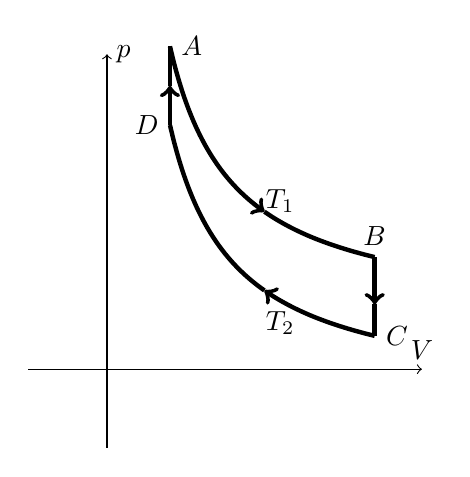
\begin{tikzpicture}[scale=2]
    \draw[->](-0.5,0)--(2,0)node[above]{$V$};
    \draw[->](0,-0.5)--(0,2)node[right]{$p$};

    \draw[->,ultra thick]plot[smooth,domain=0.4:1](\x,{0.3+0.7/(\x)});   
    \draw[-,ultra thick]plot[smooth,domain=1:1.7](\x,{0.3+0.7/(\x)});
    \draw[-,ultra thick]plot[smooth,domain=0.4:1](\x,{-0.2+0.7/(\x)});   
    \draw[<-,ultra thick]plot[smooth,domain=1:1.7](\x,{-0.2+0.7/(\x)});
    \draw[->,ultra thick](0.4,1.55)node[left]{$D$}--(0.4,1.80);
    \draw[-,ultra thick](0.4,1.8)--(0.4,2.05)node[right]{$A$};
    \draw[->,ultra thick](1.7,0.711)node[above]{$B$}--(1.7,0.411);
    \draw[-,ultra thick](1.7,0.411)--(1.7,0.211)node[right]{$C$};
    \node[above]at(1.1,0.93){$T_1$};
    \node[below]at(1.1,0.43){$T_2$};
\end{tikzpicture}
\end{document}